\documentclass[final,5p]{elsarticle}

\usepackage{amsmath}
\usepackage{amssymb}
\usepackage{graphicx}
\usepackage{booktabs}
\usepackage{array}
\usepackage{longtable}
\usepackage{url}
\usepackage{xcolor}
\usepackage{xspace}
\usepackage{listings}
\usepackage[hidelinks]{hyperref}

\journal{Journal of Systems and Software}

\newcommand{\tool}{DSC-Guard\xspace}
\newcommand{\etal}{et al.}
\newcommand{\code}[1]{\texttt{#1}}

\begin{document}

\begin{frontmatter}

\title{Semantic Log Replay for Detecting Price-Oracle Consumption Failures in EVM Lending Protocols}

\author[inst1]{Anonymous Author(s)}
\address[inst1]{Anonymous Institution}

\begin{abstract}
Price oracles are integration points between decentralized finance (DeFi) protocols and external market data.
When a lending protocol consumes a price feed with the wrong asset identity, the wrong price-composition formula, or stale temporal semantics, the resulting software state can authorize borrowing or liquidation actions that violate the protocol's economic invariants.
Existing oracle-analysis work has mainly studied transaction-level price manipulation or source-code-level feed misuse, while production incidents often leave their most reproducible evidence in contract logs.
This paper presents \tool, a log-semantics replay approach for detecting price-oracle consumption failures in EVM lending protocols.
\tool extracts log-related semantics from verified Solidity contracts with Slither, binds decoded logs to semantic roles such as oracle-boundary updates and lending impacts, and replays the resulting trace with K-style state-machine constraints for feed identity, price composition, and freshness handling.

We deliberately narrow the scope from general decentralized-oracle attacks to a recurring software-engineering failure class: oracle-consumption failures in EVM lending systems.
We evaluate \tool on six historical incidents across Ethereum, BNB Chain, Base, and Avalanche: Ploutos Money, Moonwell cbETH, Moonwell wrsETH, Blueberry, Venus LUNA, and Blizz LUNA.
The evaluation uses 470 materialized positive semantic log records, 285 impact transactions, and 10,000 case-aware benign samples that share oracle, protocol, topic, or log-shape characteristics with the incidents.
\tool detects all six incidents and all 285 impact transactions.
At log granularity, it produces 431 incident warnings over 470 incident semantic records, yielding 91.70\% incident-log warning recall with a 95\% Wilson interval of 88.86\%--93.87\%.
On 9,651 labelled benign samples, \tool produces no confirmed replayable attack false positives; 349 unresolved rows are excluded from the false-positive denominator.
An ablation study shows that removing log-semantics binding eliminates replayable detection, while oracle-only and topic-only baselines either miss downstream impacts or flood the benign set with warnings.
These results suggest that semantic log replay is a practical middle ground between raw transaction monitoring and complete EVM-level verification for a bounded but important class of DeFi software failures.
\end{abstract}

\begin{keyword}
Smart contracts \sep log analysis \sep price oracles \sep DeFi lending \sep static analysis \sep semantic replay
\end{keyword}

\end{frontmatter}

\section{Introduction}

Modern DeFi lending protocols are software systems whose correctness depends on external price-oracle integrations.
A lending market typically maps each collateral asset to one or more oracle contracts, transforms returned oracle values into a normalized price, and uses the result to compute borrow capacity or liquidation eligibility.
Failures in this integration can be catastrophic.
If a stablecoin is bound to a Bitcoin price feed, an Ether placeholder is mapped to a wrapped-Bitcoin feed, a derivative-asset oracle omits a required composition term, or a protocol keeps accepting collateral after a feed becomes stale or hits a circuit-breaker bound, the protocol's state transitions remain valid EVM executions but violate the intended lending semantics.

Prior work has studied oracle manipulation, DeFi price attacks, and source-code detection of unexpected price feeds \cite{mo2023toward,wu2021defiranger,liu2021first,kaleem2021demystifying}.
However, incident reconstruction in DeFi is often log-centric.
Protocol teams, auditors, and researchers usually reconstruct a failure from event logs, transaction receipts, governance execution records, token-transfer logs, and lending events.
Raw logs, however, are not enough.
An ABI decoder can recover event names and arguments, but it does not explain whether a log records an oracle-boundary update, whether an address is an asset or a feed, whether a borrow uses stale collateral, or whether a user address is an attacker candidate.
Conversely, full EVM semantics can be too expensive and too broad when the research question is a specific integration-level failure class.

These observations lead to three design requirements for a log-centric oracle-consumption detector.
First, the evaluation should span multiple failure modes rather than a single market-wide incident.
Second, detection effectiveness should be measured against both positive incidents and hard benign logs, rather than only by counting anomalous logs inside known attacks.
Third, the model should make explicit how multi-contract evidence, temporal order, and log incompleteness affect the soundness of replay-based detection.
We therefore narrow the problem, strengthen the dataset, and make the claims precise.
We study \emph{price-oracle consumption failures in EVM lending protocols}: historical incidents where a lending protocol consumes external oracle information with incorrect identity, transformation, or freshness semantics.
This scope is narrower than all oracle attacks, but it covers multiple real incidents and admits reproducible log-driven evidence.
Figure~\ref{fig:intro-oracle-scope-trend} shows that the corresponding oracle-scope activity on the active case chains has grown substantially over time.
The broad index-level surface is large, so the local detector materializes only evidence-closed replay slices rather than downloading every remote log.

\begin{figure}[t]
    \centering
    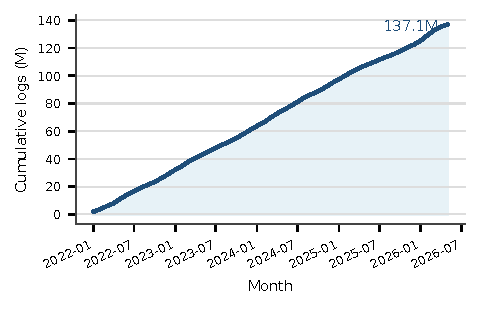
\includegraphics[width=\linewidth]{figures/intro_oracle_scope_trend.pdf}
    \caption{Cumulative oracle-scope logs on the active case chains. The trend motivates a broad index-level search surface, while local replay remains limited to materialized evidence slices.}
    \label{fig:intro-oracle-scope-trend}
\end{figure}

We present \tool, a semantic log replay tool for this scope.
\tool first extracts log-related semantic information from verified Solidity sources using Slither \cite{feist2019slither}.
It then binds decoded logs to protocol roles, including oracle boundary events, oracle anomaly markers, supply, borrow, and liquidation effects.
Finally, it replays the semantic log trace with K-style state-machine constraints inspired by rewriting-logic semantics \cite{rosu2017k,hildenbrandt2018kevm}.
The implementation does not claim complete EVM soundness.
Instead, it targets the Solidity and log subset needed to replay oracle-consumption constraints for lending protocols.

We evaluate \tool on six incidents across four EVM chains and three failure classes:
feed-binding failures, price-composition or price-semantics failures, and freshness-handling failures.
We also construct a 10,000-row benign evaluation set from case-aware oracle-scope logs.
The benign set intentionally contains hard negatives: same-oracle updates, same-protocol logs, and cross-protocol oracle-scope logs that resemble the positive cases but should not violate the replay constraints.
This design directly addresses the concern that a detector evaluated only on positive incidents can appear artificially perfect.

This paper makes the following contributions:
\begin{itemize}
    \item We define a bounded software-engineering failure class, price-oracle consumption failures in EVM lending protocols, and classify it into feed-binding, price-composition, and freshness-handling failures.
    \item We design a semantic log replay architecture that combines Slither-derived log semantics, ABI decoding, protocol-role binding, and K-style oracle-consumption constraints.
    \item We build a reproducible evidence dataset with six historical incidents, 470 positive semantic log records, 285 impact transactions, 55 actor candidates, and 10,000 case-aware benign samples.
    \item We report standard detection metrics, early-evidence lead time, attacker-candidate localization, and ablation results. \tool detects all six incidents and all 285 impact transactions, achieves 91.70\% incident-log warning recall, and has no false positives among 9,651 labelled benign samples.
    \item We explicitly discuss limitations: logs may omit state changes, constraints are failure-class-specific, and the tool is not a universal oracle-attack detector or a full EVM verifier.
\end{itemize}

\section{Background}
\label{sec:background}

\subsection{Price Oracles and Lending Protocols}

EVM lending protocols consume external price data through oracle contracts.
Figure~\ref{fig:oracle-workflow} shows the basic data-feed pattern represented by Chainlink-style oracle systems.
An oracle network publishes price observations to an aggregator or feed contract.
A consumer protocol, such as a lending market or oracle wrapper, reads the feed through an interface or proxy and transforms the returned answer into a normalized asset price.
The lending protocol then uses this price to compute collateral value, borrow capacity, liquidation eligibility, and market-risk checks.

\begin{figure}[t]
    \centering
    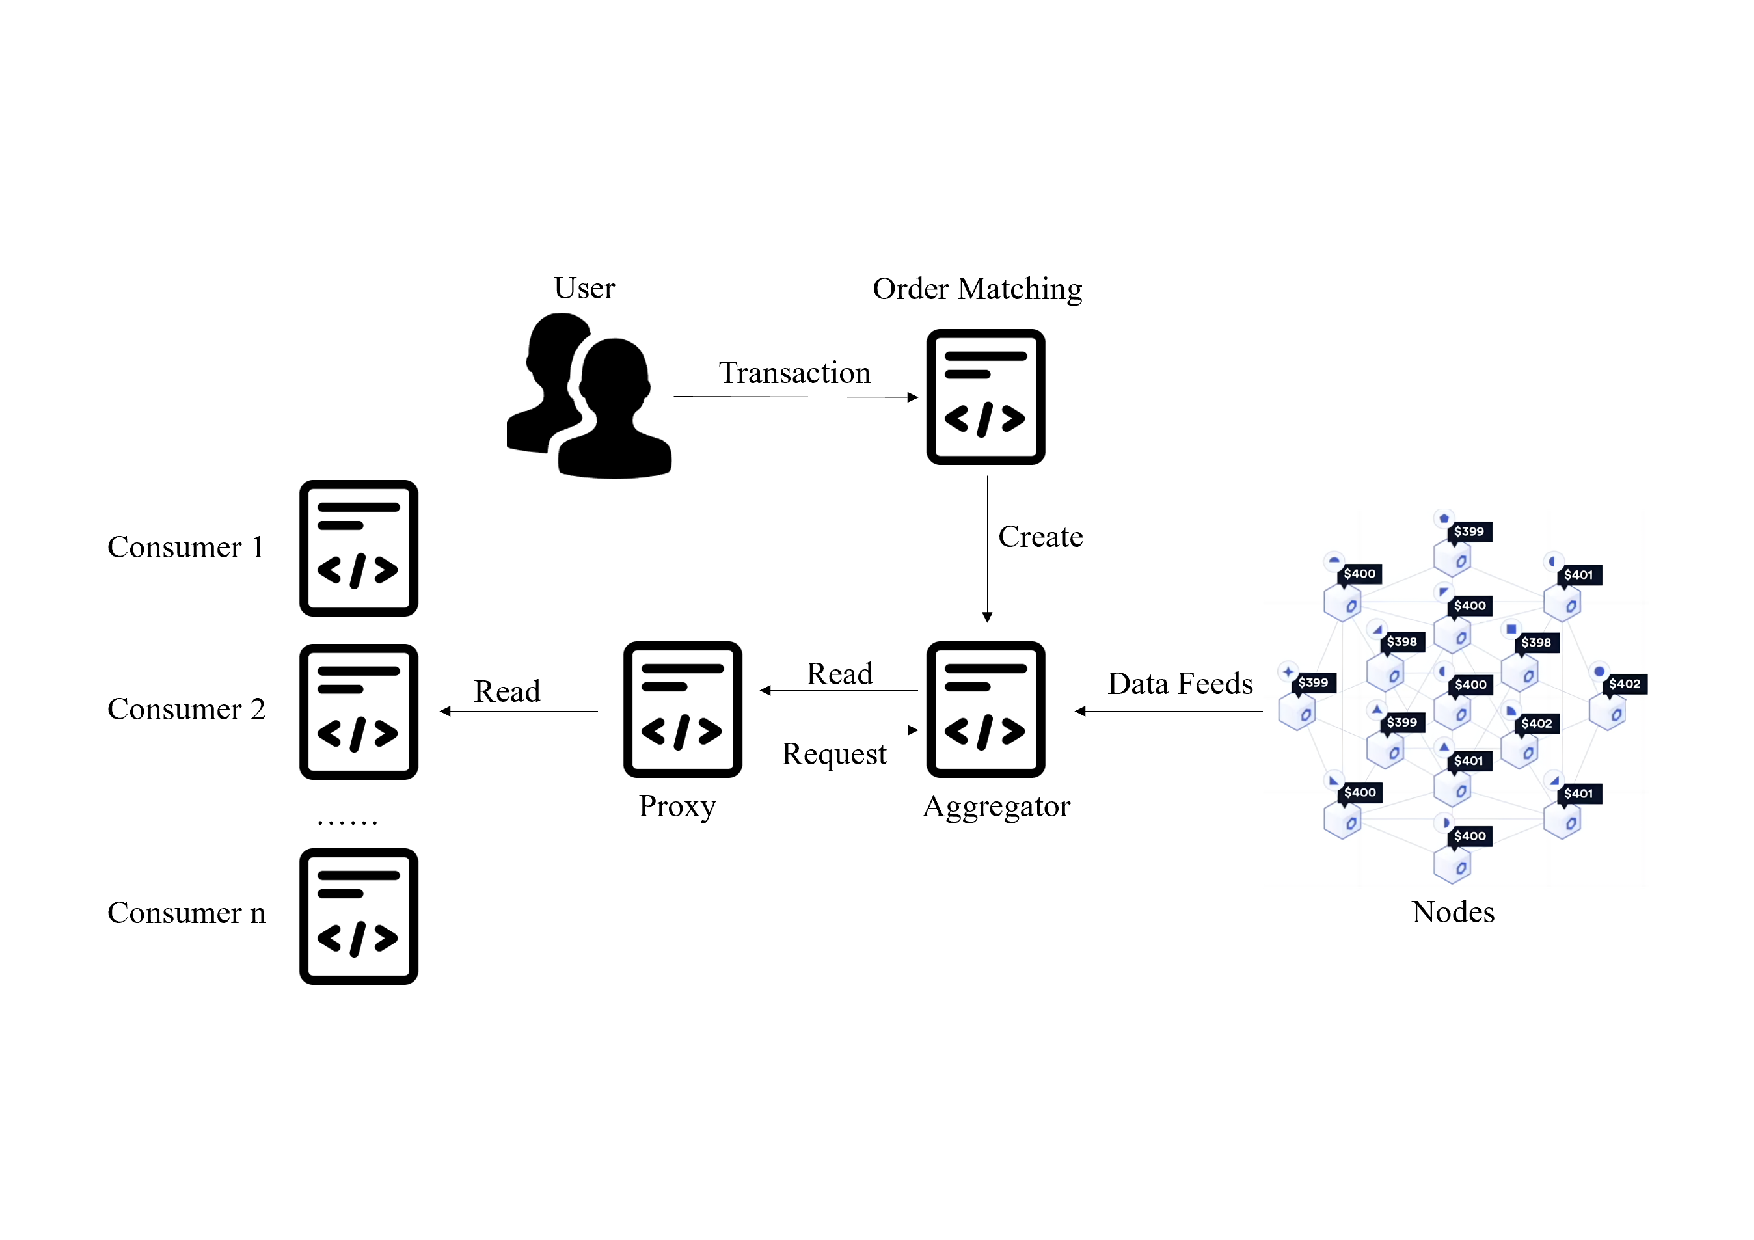
\includegraphics[width=\linewidth]{figures/DON_workflow.pdf}
    \caption{Chainlink-style price-oracle workflow. The revised scope focuses on the consumer side: how EVM lending protocols bind, transform, and validate oracle values before borrow or liquidation decisions.}
    \label{fig:oracle-workflow}
\end{figure}

This pipeline creates an integration boundary.
The oracle feed can be correctly reporting its own value, while the consumer protocol still fails if it binds the wrong asset to the feed, applies the wrong price-composition formula, or keeps using a stale or circuit-breaker value.
For this reason, DSC-Guard does not treat oracle logs in isolation.
It connects oracle-boundary evidence to downstream lending logs such as supply, borrow, and liquidation.

\subsection{Smart Contract Logs}

Smart contract logs are structured records emitted by contracts during transaction execution.
They are stored in transaction receipts and consist of an emitting contract address, indexed topics, unindexed data, block and transaction metadata, and a log index.
The first topic is usually the hash of the event signature, while the remaining topics contain indexed event parameters.
Unindexed parameters are ABI-encoded in the data field.
Figure~\ref{fig:log-example} shows an example of decoded blockchain logs.

\begin{figure}[t]
    \centering
    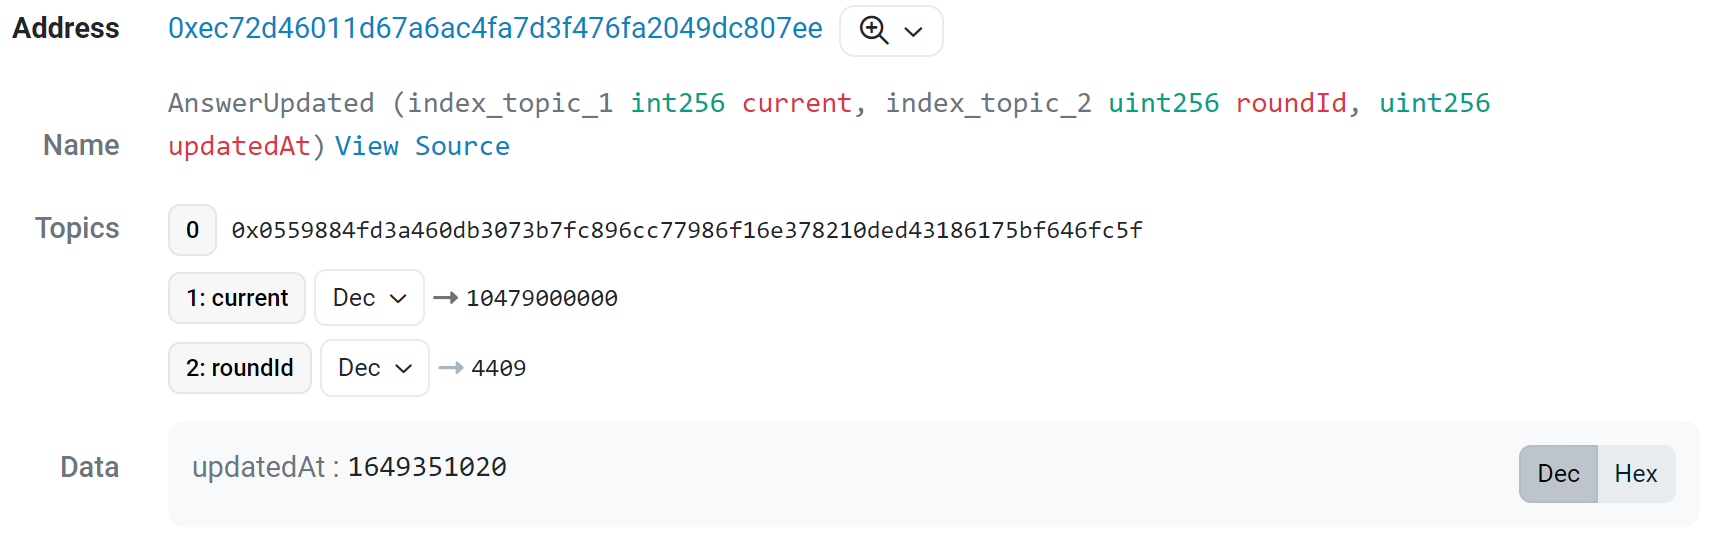
\includegraphics[width=\linewidth]{figures/log_example.png}
    \caption{Example of decoded blockchain logs. DSC-Guard uses raw receipt order, event topics, ABI fields, and source-derived semantic roles to construct replay records.}
    \label{fig:log-example}
\end{figure}

Solidity contracts declare events with the \code{event} keyword and emit them with \code{emit}.
An ABI decoder can recover event names and typed parameters from receipts when the contract ABI is available.
However, ABI decoding alone does not recover the semantic role of a log.
For example, an address parameter may denote an actor, an asset, a feed, a market token, an implementation contract, or a recipient.
Similarly, a log may indicate a harmless price update, an oracle-boundary change, a collateral-enabling supply, or a downstream impact.
DSC-Guard therefore combines ABI-decoded logs with source-derived semantics and protocol-level evidence closure.

\section{Scope and Failure Model}
\label{sec:scope}

\subsection{Oracle-Consumption Failures}

We focus on \emph{oracle-consumption failures}: incidents where a lending protocol incorrectly consumes price-oracle information when computing collateral value, borrow capacity, or liquidation eligibility.
These failures are difficult because the suspicious behavior is not necessarily in the oracle feed itself.
The external oracle may report a valid value, and each individual transaction may be a valid EVM execution.
The failure emerges only when protocol-side source semantics, historical logs, asset/feed identity, temporal order, and downstream lending impact are interpreted together.

This scope is different from both generic smart-contract vulnerability detection and market-side price manipulation.
Generic smart-contract tools and surveys study vulnerabilities such as reentrancy, overflow, authorization mistakes, and delegatecall misuse \cite{vidal2024slr,iuliano2026slr}.
Price-manipulation detectors reason about how attackers move market prices through swaps, liquidity changes, or transaction-level token flows \cite{wu2021defiranger,zhong2025defiscope}.
Our failure model is complementary: the price may be externally valid, but the lending protocol consumes it with incorrect identity, transformation, or freshness semantics.
We therefore exclude flash-loan manipulation of DEX prices, sandwiching, bridge-message failures, randomness oracles, and general market-wide price discovery.

\subsection{Why These Failures Are Hard to Detect}

A detector for this scope must solve several semantic problems that are not visible from a single event topic or a single transaction.
\textbf{Consumer-side hiddenness} means that a feed can be normal while the consumer protocol binds it to the wrong asset, omits a required composition term, or ignores freshness semantics.
\textbf{ABI semantic gap} means that ABI decoding recovers field names and values but not whether an address is an actor, asset, feed, market token, implementation contract, or recipient.
\textbf{Multi-contract evidence} means that the trigger, oracle wrapper, market token, ERC20 transfer, borrow, and liquidation logs may be emitted by different contracts in the same protocol cluster.
\textbf{Temporal causality} means that dangerous oracle-boundary evidence and downstream impact may be separated by multiple blocks or transactions, so detection requires a boundary-to-impact order rather than same-transaction matching.
\textbf{Benign look-alikes} mean that normal oracle updates, supplies, borrows, and liquidations often share the same topics and event names as attack-chain logs.

These challenges explain why existing approaches are not directly sufficient for the evidence closure studied here.
VeriOracle targets source-level unexpected price-feed usage \cite{mo2023toward}, but our evaluation requires historical log materialization, temporal replay, and actor localization.
DeFiRanger and DeFiScope target price-manipulation behavior and transaction-level price-model reasoning \cite{wu2021defiranger,zhong2025defiscope}, whereas our cases require modeling how lending protocols consume oracle values after configuration, wrapper, or freshness failures.
ABI-only or topic-only log parsing is also insufficient because it cannot recover the replay roles needed to distinguish a benign \code{AnswerUpdated} or \code{SUPPLY} log from dangerous evidence.

\subsection{Failure Classes}

We classify oracle-consumption failures by the semantic contract violated at the consumer protocol boundary.
This classification is useful for software engineering because each class maps to a specific integration obligation in the lending pipeline.

\begin{description}
    \item[Feed-binding failure.] The violated contract is asset identity. The protocol maps an asset to an unrelated price source, such as USDC being treated as if it were backed by a BTC/USD feed.
    \item[Price-composition failure.] The violated contract is price transformation. The protocol reads the right kind of oracle component but applies an incomplete or wrong formula, such as valuing a derivative asset without multiplying by the required base-asset USD price.
    \item[Freshness-handling failure.] The violated contract is temporal validity. The protocol keeps accepting collateral after a feed becomes stale, paused, lower-bounded, or otherwise economically invalid for lending decisions.
\end{description}

The three classes require different evidence.
Feed-binding and price-composition failures require protocol-side configuration or wrapper semantics, so Chainlink \code{AnswerUpdated} logs alone are not enough.
Freshness-handling failures require oracle update history, but they still become security-relevant only when connected to downstream lending behavior such as collateral supply, borrow, or liquidation.

\subsection{Log-Centric Evidence Closure}

Our unit of evidence is a semantic log record.
A record contains the transaction hash, block metadata, event type, decoded parameters, and role annotations such as \code{oracle\_boundary}, \code{supply}, \code{borrow}, \code{liquidation}, or \code{early\_evidence}.
The same transaction can generate multiple logs, but the replay model treats each semantic record as a state transition.
DSC-Guard therefore does not flag a candidate because one log looks suspicious.
It treats a candidate as replayable only when oracle-boundary evidence, protocol-side impact, actor-bearing logs, temporal order, and a violated oracle-consumption constraint are jointly observable.

We distinguish three log roles in evaluation:
\begin{description}
    \item[Direct violation logs.] Oracle anomaly markers and downstream borrow/liquidation logs expected to trigger a replay constraint.
    \item[Collateral-enabling early-evidence logs.] Supply logs that occur after a bad-oracle state is active and are causally connected to a later same-actor borrow or liquidation impact.
    \item[Support-only context logs.] Logs needed to preserve replay context but not expected to trigger a warning.
\end{description}
This distinction prevents two misleading extremes.
Counting only direct violation logs makes log-level recall look trivially perfect.
Counting every supply log as a warning makes the detector look overfitted.
Our current implementation marks a supply log as early evidence only when it satisfies an evidence-closure gate: affected collateral asset, active bad-oracle state, same actor, temporal order, and a later lending impact.
This is why the same event type can be benign in one context and dangerous in another.
For example, \code{AnswerUpdated} is usually a normal feed update, but it can become part of a stale-oracle episode if no valid update follows before lending impact.
Similarly, \code{SUPPLY} is normal lending activity unless it supplies an affected collateral asset after an oracle anomaly and before a same-actor borrow or liquidation.

\section{Method}
\label{sec:method}

\subsection{Overview}

\tool has five stages:
\begin{enumerate}
    \item \textbf{Source collection.} For each case, the collector stores verified Solidity sources, ABI files, proxy/implementation metadata when available, and known incident transactions.
    \item \textbf{Semantic mining.} Slither is used to extract event declarations, emitted events, state variables, mapping updates, external calls, and data dependencies around oracle reads and lending actions.
    \item \textbf{Log binding.} The joint parser decodes receipts and Dune-exported events with ABI information, then binds them to semantic roles such as \code{ORACLE\_FEED\_SET}, \code{STALE\_ORACLE\_START}, \code{SUPPLY}, \code{BORROW}, and \code{LIQUIDATE}.
    \item \textbf{K-style replay.} The replay engine maintains abstract cells for oracle maps, stale assets, formula violations, market state, positions, balances, and alerts. It checks replay constraints over the ordered semantic trace.
    \item \textbf{Localization and reporting.} The verifier emits alerts, actor candidates, evidence transaction hashes, and case reports.
\end{enumerate}

\begin{figure}[t]
    \centering
    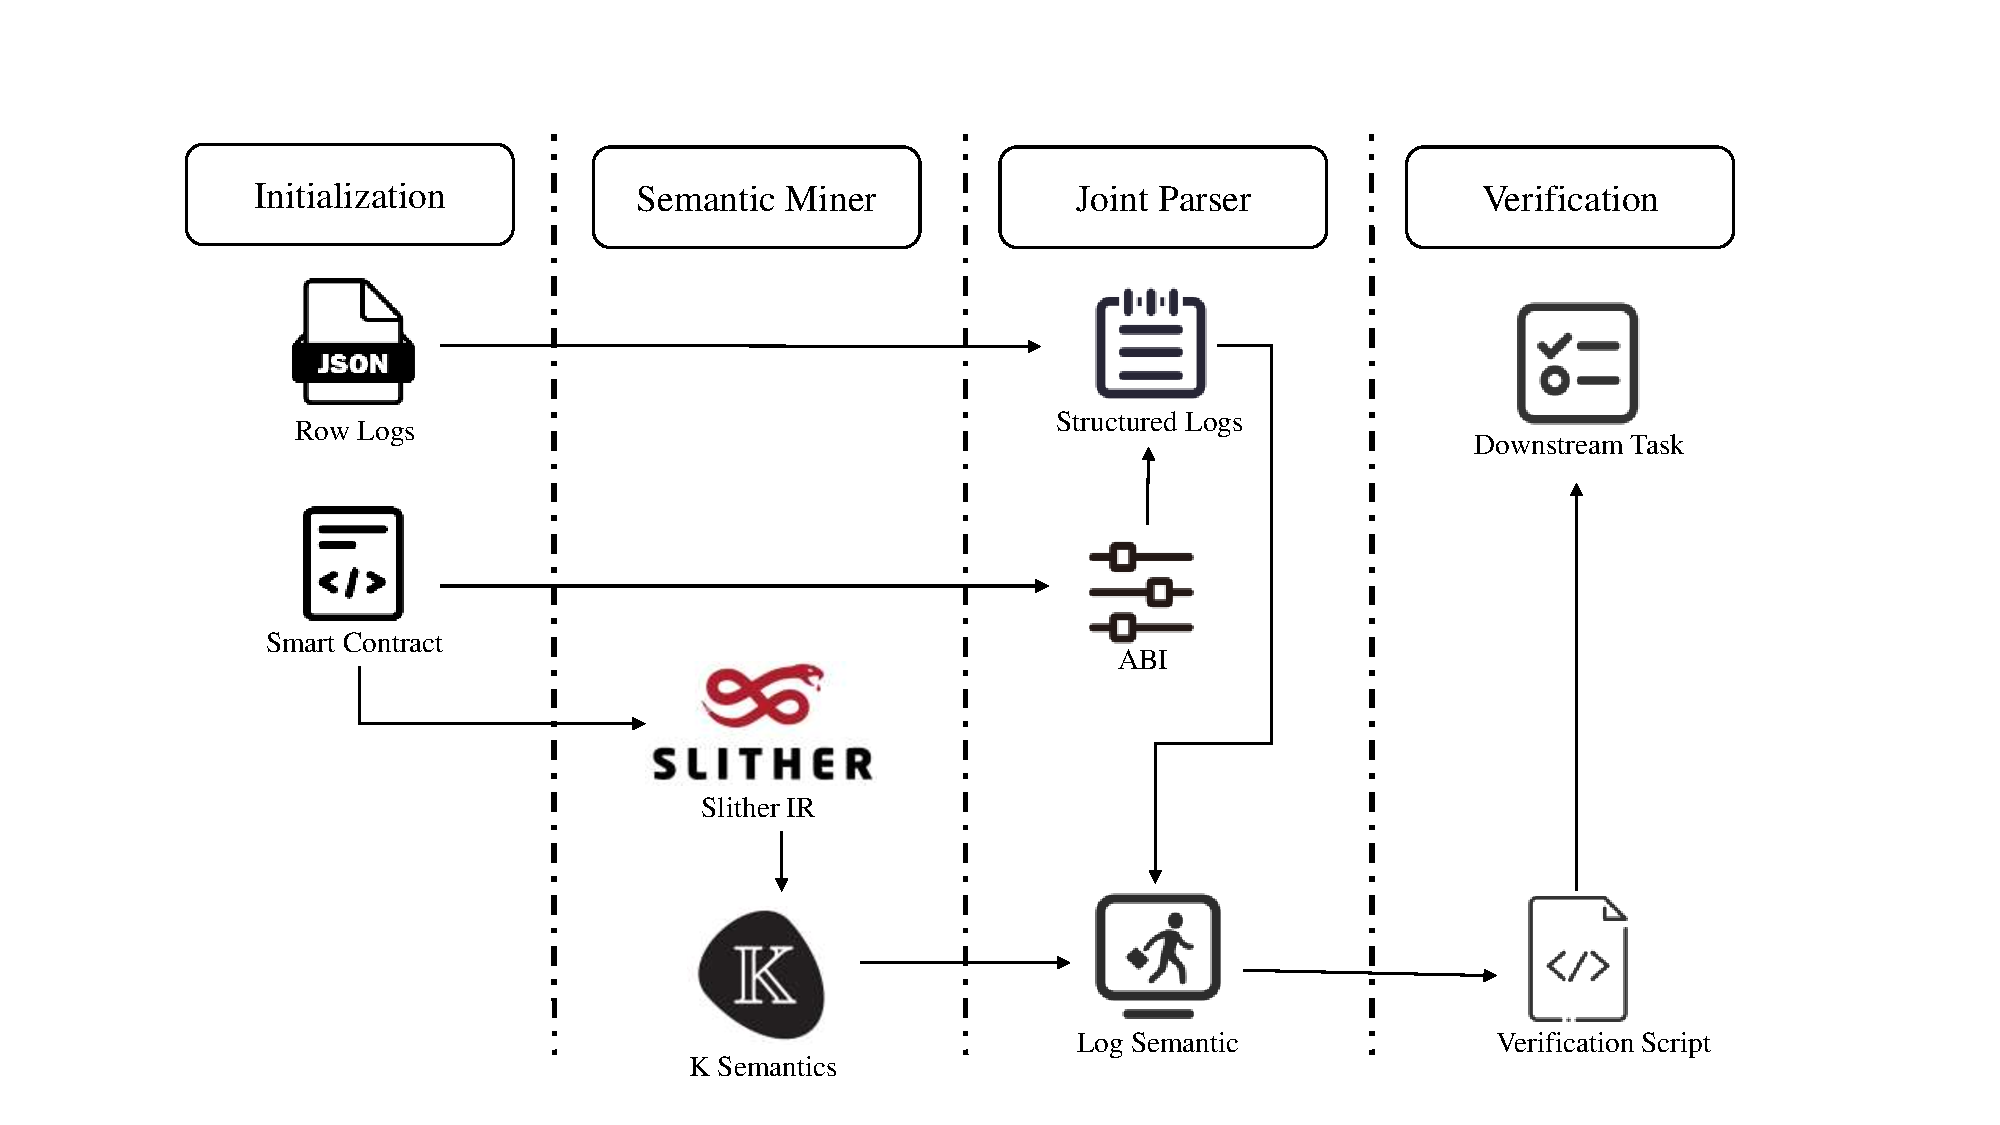
\includegraphics[width=\linewidth]{figures/tool_workflow.pdf}
    \caption{Workflow of DSC-Guard. The original workflow is retained, but the revised paper constrains the target semantics to EVM lending oracle-consumption failures rather than general DON attacks.}
    \label{fig:workflow}
\end{figure}

The design deliberately avoids global DeFi-state modeling.
\tool does not attempt to symbolically execute all contracts in a transaction or model every composable protocol.
Instead, it extracts a bounded trace around contracts and logs relevant to oracle consumption and lending impacts.
This is a pragmatic compromise: cross-contract dependencies are represented when they are observable in the evidence closure, but unlogged internal state changes remain a limitation.
Figure~\ref{fig:workflow} shows the end-to-end workflow.
Compared with the previous DON-oriented version, the revised workflow narrows the semantic boundary at two points.
First, the semantic miner only retains source-code paths that affect oracle boundary logs or lending-state logs.
Second, the verifier checks oracle-consumption constraints rather than arbitrary data-feed anomalies.
This makes the replay state small enough to be executed over materialized historical traces while still preserving the cross-contract evidence needed for oracle, market, token, and actor relationships.

\subsection{Semantic Miner}

The semantic miner recovers log-related program semantics from Solidity sources.
For each verified contract, it identifies event declarations and emission sites, then uses Slither's AST, CFG, SlithIR, and state-variable read/write information to extract:
\begin{itemize}
    \item event name and argument roles;
    \item state variables updated near emitted logs;
    \item oracle setter and oracle read functions;
    \item market actions such as supply, borrow, redeem, repay, liquidation, and collateral-entry events;
    \item temporal checks such as \code{updatedAt}, \code{roundId}, and heartbeat-style freshness logic when present.
\end{itemize}
The miner outputs a compact semantic IR rather than a full contract model.
When source code or ABI metadata is incomplete, the tool marks the evidence quality explicitly, such as \code{receipt\_flow\_decoded} or \code{manual-seed-supported}, instead of silently treating the case as fully source-derived.

\begin{figure}[t]
    \centering
    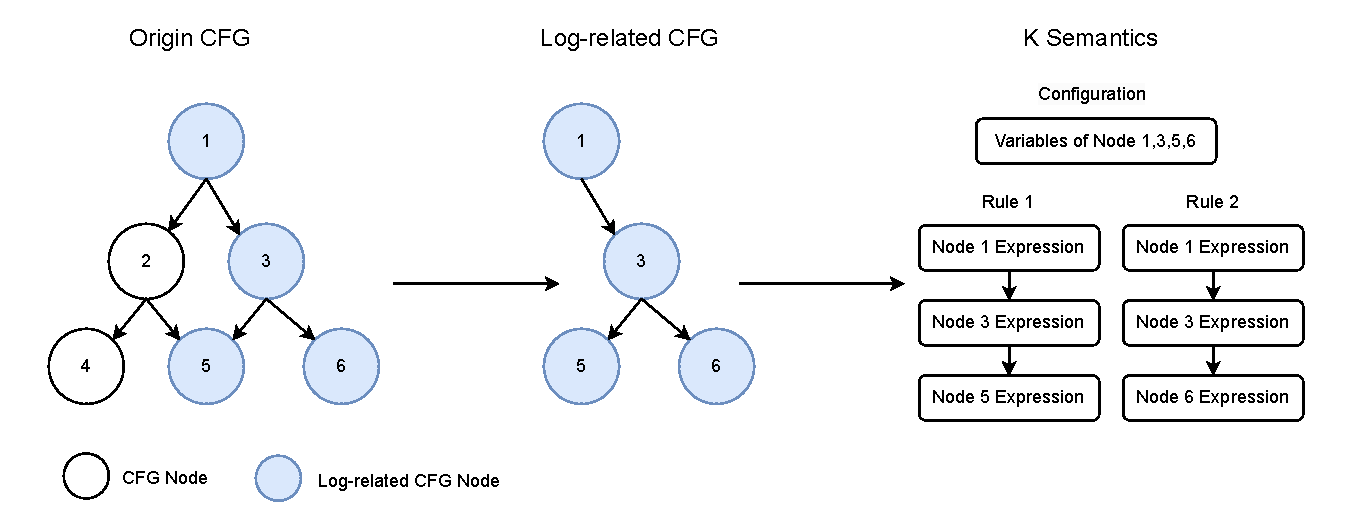
\includegraphics[width=\linewidth]{figures/semantic_miner.pdf}
    \caption{Semantic mining workflow inherited from the original DSC-Guard design. In the JSS revision, the mined semantics are restricted to oracle-boundary events, oracle reads, lending actions, and actor-bearing impact logs.}
    \label{fig:semantic-miner}
\end{figure}

Figure~\ref{fig:semantic-miner} illustrates the semantic mining step.
For each event declaration, the miner first records the event signature, indexed fields, non-indexed fields, and emission sites.
For each emission site, it builds a function-level control-flow graph from Slither IR and computes a backward dependency slice from the emitted event arguments, modified storage variables, oracle-read return values, and lending-action arguments.
Nodes that neither reach the emitted log nor update a replay-relevant state variable are removed from the pruned CFG.
The remaining nodes are translated into a case-independent semantic IR with the following fields:

\begin{lstlisting}[basicstyle=\footnotesize\ttfamily,breaklines=true]
{
  "event": "Borrow",
  "entry_function": "borrowFresh",
  "semantic_role": "BORROW",
  "actor_fields": ["borrower", "sender"],
  "asset_fields": ["market", "underlying"],
  "state_reads": ["oracle", "accountBorrows"],
  "state_writes": ["totalBorrows", "accountBorrows"],
  "oracle_reads": ["getUnderlyingPrice"],
  "freshness_checks": ["updatedAt", "answeredInRound"],
  "evidence_quality": "slither_ir"
}
\end{lstlisting}

The pruning criterion is intentionally role-oriented rather than whole-program-oriented.
For feed-binding failures, the retained slice must include asset-to-source mapping writes or oracle setter events.
For price-composition failures, the retained slice must include price-wrapper configuration, exchange-rate usage, or transformation logic.
For freshness-handling failures, the retained slice must include Chainlink answer fields, freshness checks when present, and downstream lending actions that consume the resulting collateral valuation.
This design is less general than whole-contract verification, but it directly supports the replay constraints evaluated in this paper.

\subsection{Joint Parser and Evidence Binding}

The joint parser binds the source-derived semantic IR to historical logs and receipts.
Its input is a time-ordered sequence of transaction receipts, ABI-decoded logs, ERC20 transfer logs, and Dune-exported decoded events.
Its output is the semantic trace replayed by the verifier.
The parser performs four binding steps.
First, it matches log \code{topic0} to an ABI event signature and decodes indexed and data fields.
Second, it matches the decoded event to a mined semantic role, such as \code{ORACLE\_FEED\_SET}, \code{SUPPLY}, \code{BORROW}, or \code{LIQUIDATE}.
Third, it normalizes chain-specific and protocol-specific addresses into asset, feed, market, actor, and protocol-cluster fields.
Fourth, it attaches evidence metadata, including transaction hash, block number, timestamp, transaction index, log index, source quality, and whether the record came from ABI decoding, Dune decoding, raw receipt flow, or manual incident seed metadata.

\begin{figure}[t]
    \centering
    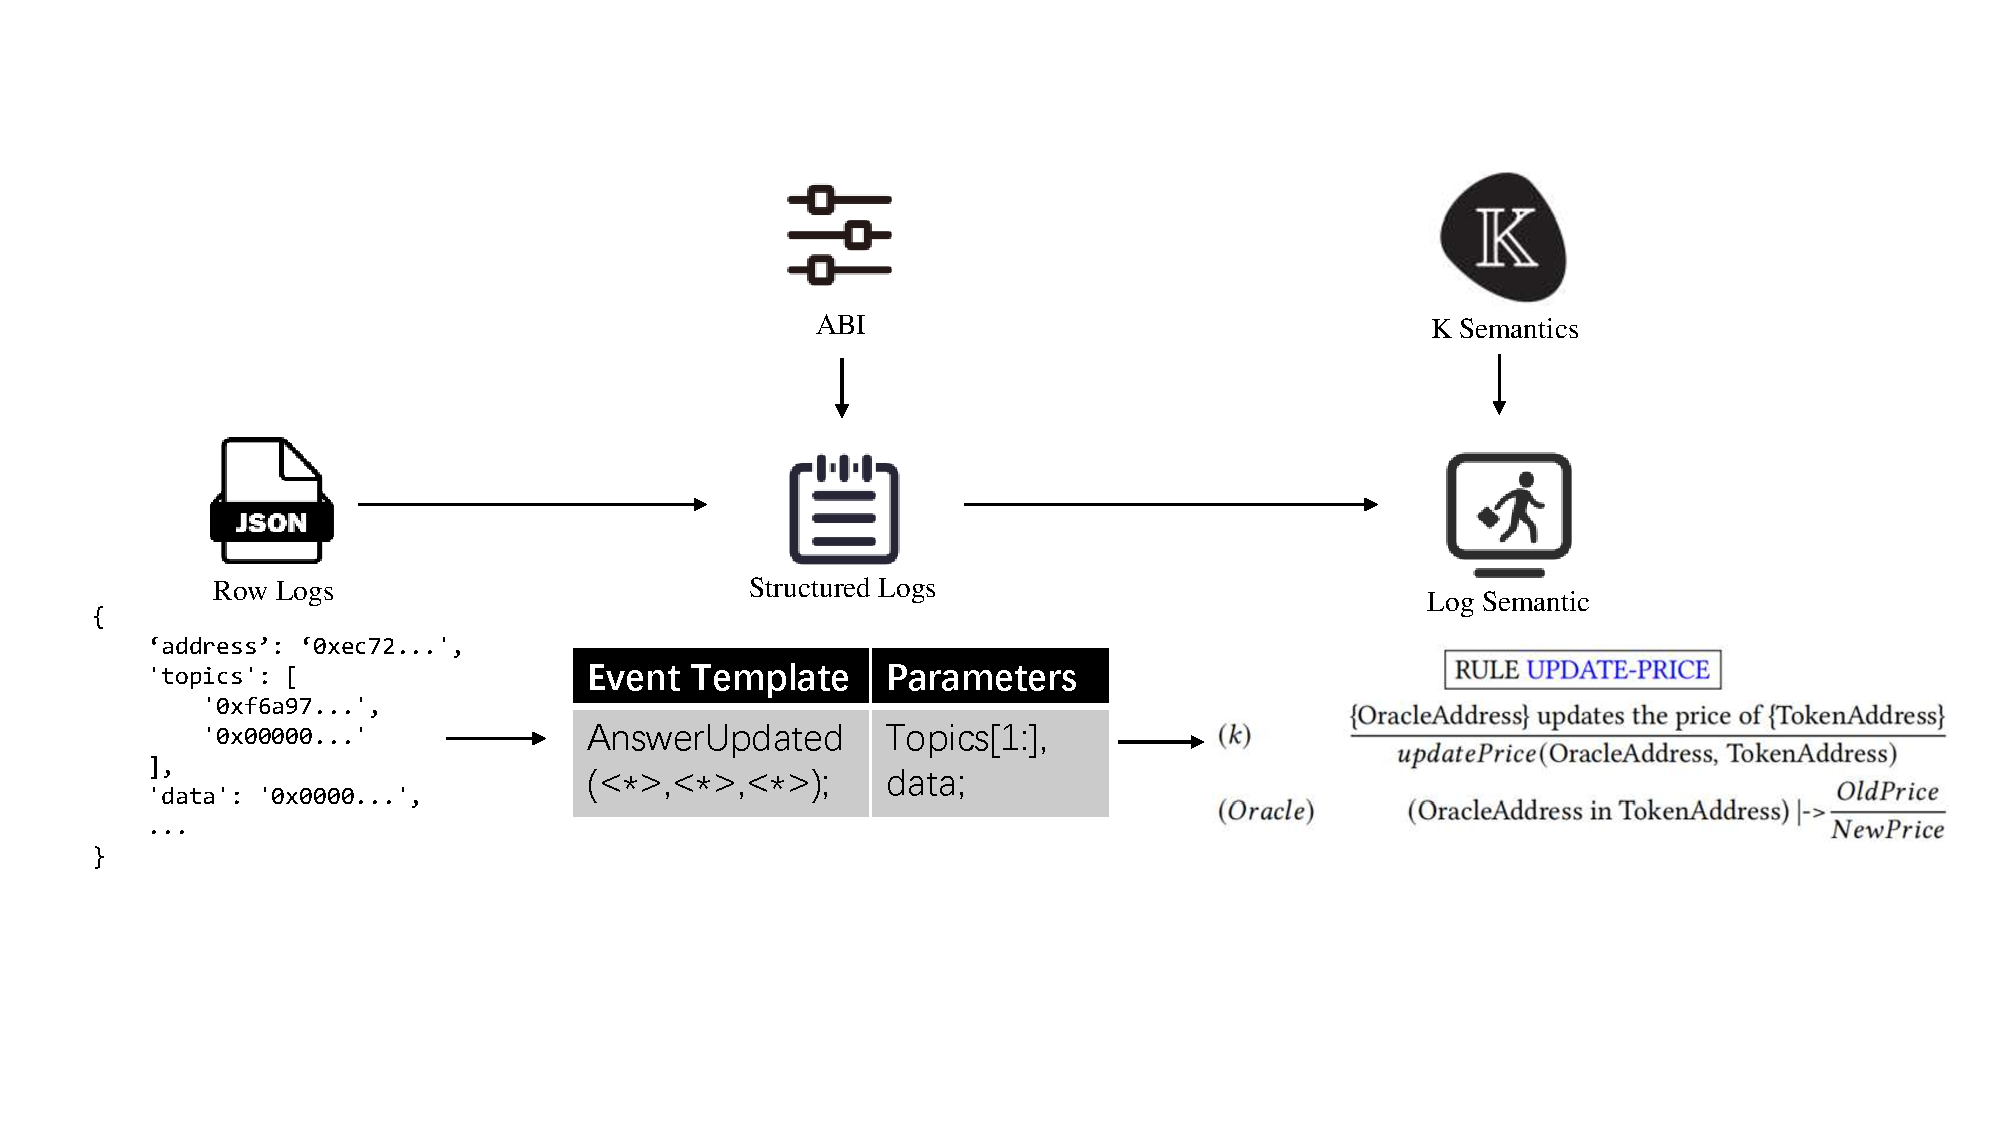
\includegraphics[width=\linewidth]{figures/joint_parser.pdf}
    \caption{Joint parser workflow. The parser connects ABI-decoded logs and source-derived semantics, then emits ordered replay statements for oracle-consumption constraints.}
    \label{fig:joint-parser}
\end{figure}

Figure~\ref{fig:log-example} shows the decoded log evidence used by the parser, and Figure~\ref{fig:joint-parser} shows the binding process.
The parser is deliberately conservative.
If a receipt contains token transfers but no protocol-level borrow event, the record may support impact-flow evidence but cannot overwrite the protocol-level \code{borrow\_amount}.
If a source contract is unavailable, the parser can still preserve raw receipt evidence and ERC20 transfer flow, but the resulting record is marked as inferred or receipt-flow-backed.
These evidence-quality tags are used in the dataset audit and prevent the evaluation from treating every historical log as fully source-derived.

The trace emitted by the joint parser has a stable schema:

\begin{lstlisting}[basicstyle=\footnotesize\ttfamily,breaklines=true]
{
  "chain": "base",
  "block_number": 123,
  "tx_hash": "0x...",
  "log_index": 7,
  "event_type": "BORROW",
  "asset": "cbETH",
  "actor": "0x...",
  "oracle_state_ref": "cbETH/USD",
  "decoded": {...},
  "evidence_quality": "dune_decoded_event"
}
\end{lstlisting}

The verifier consumes only this normalized semantic trace.
This separation makes it possible to compare full DSC-Guard with ablations: an ABI-only parser can decode event fields but lacks semantic roles and evidence closure; a topic-only parser can match topics but cannot decide whether a log represents oracle consumption, collateral enabling, or benign protocol activity.

\subsection{K-Style Replay Semantics}

The replay state has abstract cells:
\[
\langle oracleMap \rangle,\quad
\langle oracleAnswer \rangle,\quad
\langle marketState \rangle,\quad
\langle positions \rangle,\quad
\langle alerts \rangle.
\]
Rules are generated for oracle boundary logs, price-composition markers, stale oracle markers, supply logs, borrow logs, and liquidation logs.
For example, a feed-binding update records an asset-to-feed mapping in \(\langle oracleMap \rangle\), and a later borrow checks whether the borrower's collateral asset is mapped to a forbidden or unexpected feed.
Similarly, a stale oracle marker records the affected asset in \(\langle oracleAnswer \rangle\), and a later borrow against that asset triggers an \code{attacker\_localization} alert.

The generated K-style module contains a small language of replay statements rather than a full Solidity or EVM semantics.
The core syntax is:

\begin{lstlisting}[basicstyle=\footnotesize\ttfamily,breaklines=true]
Block ::= Statement ";" | Block Statement ";"
Statement ::= "exec(" Log ")" | "DONE" | "FAIL"
Log ::= ORACLE_BOUNDARY | ORACLE_ANOMALY
      | SUPPLY | BORROW | LIQUIDATE | TRANSFER
\end{lstlisting}

During replay, each semantic log is rewritten against the configuration cells.
An oracle-boundary log updates \(\langle oracleMap \rangle\) or \(\langle oracleAnswer \rangle\).
A supply log updates \(\langle positions \rangle\) and may create a collateral-enabling warning if a bad-oracle state is already active and the same actor later produces an impact log.
A borrow or liquidation log checks the active oracle state, records violated constraints, and emits actor candidates.
The replay therefore models the state changes needed for the evaluated failure class, while explicitly excluding unrelated EVM state.

The replay constraints used in this study are:
\begin{itemize}
    \item an asset must not be mapped to an unrelated feed, such as USDC mapped to BTC/USD;
    \item derivative-asset prices must satisfy expected composition semantics, such as cbETH/USD requiring cbETH/ETH multiplied by ETH/USD;
    \item stale or lower-bound oracle values must not be consumed as borrowable collateral;
    \item borrowing impact after an oracle violation identifies borrower, liquidator, sender, or recipient fields as actor candidates;
    \item supply logs under an active oracle anomaly become early evidence only when they enable or materially increase bad-oracle collateral capacity for a later same-actor impact.
\end{itemize}

\subsection{Why Logs Instead of Full EVM State?}

Logs provide stable, compact, and publicly indexed evidence, but they are not complete state.
This paper uses logs because they are the common substrate for incident response and cross-chain historical analysis.
However, our soundness claim is intentionally limited.
If a contract silently mutates a price source or account position without emitting a relevant event, a log-only state machine can desynchronize from the actual EVM state.
The implementation partially mitigates this by using source semantics and raw receipts, but it does not eliminate the blind spot.
We treat this as a limitation rather than an assumption hidden in the model.

\section{Dataset and Experimental Design}
\label{sec:dataset}

Figure~\ref{fig:dataset-funnel} summarizes the evaluation funnel.
The broad oracle-scope surface is kept as an index-level coverage artifact, while local replay focuses on the positive incident traces and case-aware benign samples needed for semantic validation.

\begin{figure}[t]
    \centering
    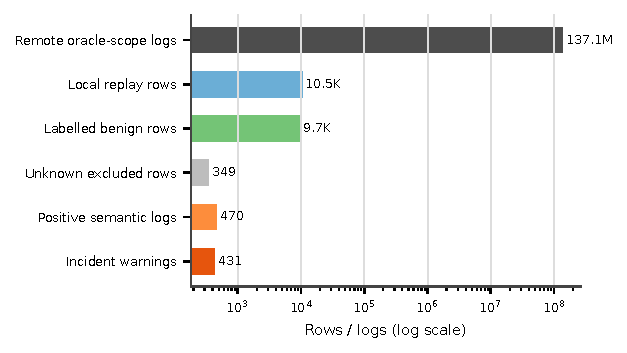
\includegraphics[width=\linewidth]{figures/eval_dataset_funnel.pdf}
    \caption{Evaluation data funnel. The broad oracle-scope count is remote index-level coverage; local replay uses materialized positive traces and benign samples with minimal evidence bundles.}
    \label{fig:dataset-funnel}
\end{figure}

\subsection{Positive Incidents}

Table~\ref{tab:cases} summarizes the six positive cases.
They span four EVM chains and three failure classes.
Five cases are fully materialized from historical events; Ploutos is backed by real transactions, raw receipts, and ERC20 transfer flow, but some protocol-specific fields remain inferred from known transactions.

\begin{table*}[t]
\centering
\caption{Positive incident dataset.}
\label{tab:cases}
\small
\begin{tabular}{lllr rrr}
\toprule
Case & Chain & Failure class & Trace records & Warnings & Impact txs & Actor candidates \\
\midrule
Ploutos Money & Ethereum & Feed binding & 4 & 3 & 1 & 1 \\
Moonwell cbETH & Base & Price composition & 124 & 124 & 123 & 14 \\
Moonwell wrsETH & Base & Price semantics & 13 & 13 & 12 & 2 \\
Blueberry & Ethereum & Price semantics & 2 & 2 & 1 & 2 \\
Venus LUNA & BNB Chain & Freshness handling & 218 & 201 & 95 & 12 \\
Blizz LUNA & Avalanche & Freshness handling & 109 & 88 & 53 & 24 \\
\midrule
Total &  &  & 470 & 431 & 285 & 55 \\
\bottomrule
\end{tabular}
\end{table*}

The incidents cover different forms of oracle-consumption failure.
Ploutos tests feed identity mismatch.
Moonwell cbETH tests price-composition semantics.
Moonwell wrsETH and Blueberry test price-semantics and implementation-level oracle mismatch.
Venus and Blizz test freshness-handling failures during the LUNA collapse.

\subsection{Benign Dataset}

\paragraph{Sampling frame}
The benign set is case-aware rather than uniformly random.
It is designed to be hard for a detector: benign samples share topics, contracts, oracle feeds, or protocol neighborhoods with the positive incidents.
Candidates are drawn from the oracle-scope surface associated with the six positive cases.
The two strata are same-oracle logs, which exercise normal updates from the same or similar feeds, and case-topic logs, which exercise configuration, oracle-wrapper, governance, or lending topics that resemble the incident traces.
We exclude the incident windows, known attack transactions, and known positive evidence paths before local materialization.

\paragraph{Sampling policy}
We generated 10,000 materialized benign samples without using Dune for local replay.
Small candidate pools are included as completely as the available evidence permits, while large pools are reduced with deterministic hash sampling over stable log identifiers.
The sampling procedure does not use top-\(k\) truncation, amount ranking, candidate scores, or nondeterministic random sampling.
Explorer and RPC evidence was cached locally, and every selected sample was replayed against the same constraints as the positive cases.

\paragraph{Labeling rule}
A sample enters the labelled benign denominator only after materialized receipt, log, source or ABI, and trace evidence support replay under the same DSC-Guard constraints.
The replay must produce no oracle-consumption violation, no attacker localization, and no match to a known positive path.
If source/ABI metadata or semantic binding is insufficient to establish this result, the row remains \code{unknown\_after\_materialization} and is excluded from the false-positive denominator.

The false-positive denominator contains 9,651 samples that were labelled benign after local materialization, replay, and artifact inspection.
Another 349 rows remain \code{unknown\_after\_materialization} because source/ABI or semantic binding was insufficient to prove a strict benign label.

\begin{table}[t]
\centering
\caption{Benign evaluation set.}
\label{tab:benign}
\small
\begin{tabular}{lrrr}
\toprule
Stratum & Total & Labelled benign & Unknown \\
\midrule
Same oracle & 6,374 & 6,374 & 0 \\
Case topic & 3,626 & 3,277 & 349 \\
\midrule
Total & 10,000 & 9,651 & 349 \\
\bottomrule
\end{tabular}
\end{table}

For transparency, the 10,000 benign samples are related to the six positive cases as follows: Venus LUNA contributes 4,751 materialized samples, Moonwell cbETH 2,896, Blizz LUNA 1,623, Moonwell wrsETH 636, Ploutos 60, and Blueberry 34.
This distribution reflects available historical oracle-scope evidence and the deterministic sampling policy rather than an attempt to match case severity or loss size.

\subsection{Research Questions}

We evaluate four research questions:
\begin{description}
    \item[RQ1 Detection effectiveness.] Can \tool detect known oracle-consumption incidents, impact transactions, and warning logs?
    \item[RQ2 Early evidence.] How early does \tool observe dangerous oracle/config/stale evidence before the first downstream impact?
    \item[RQ3 Actor localization.] Can \tool identify the actors associated with borrow or liquidation impact logs?
    \item[RQ4 Ablation.] Which semantic components are necessary for replayable detection?
\end{description}

We report case-level recall, transaction-level recall, log-level warning recall, precision over labelled benign samples, lead time, actor recall, and ablation metrics.

\section{Evaluation}
\label{sec:evaluation}

\subsection{RQ1: Detection Effectiveness}

\paragraph{Experiment design}
To answer RQ1, we replay the six positive incident traces and the 10,000 materialized benign samples with the same verifier configuration.
The positive traces contain oracle-boundary records, oracle-anomaly records, lending supply and borrow records, liquidation records, and context records needed to preserve replay state.
The benign samples are case-aware hard negatives drawn from similar oracle and lending activity outside the incident paths.
This design evaluates whether \tool can detect known failures without treating ordinary oracle updates, supply operations, or borrow transactions as attacks.

\paragraph{Metrics}
We report detection at three granularities.
Case-level recall asks whether each historical incident is detected.
Impact-transaction recall asks whether the materialized borrow and liquidation transactions in the positive traces are flagged.
Log-level warning recall is computed over 470 positive semantic records, which include direct violation targets, collateral-enabling early-evidence records, and support-only context records.
Only the first two categories are expected to raise warnings; the support-only records remain in the denominator to avoid a target-only recall metric.
For benign data, we report false positives over 9,651 labelled benign samples; the remaining 349 unknown rows are excluded from the false-positive denominator.

\begin{table}[t]
\centering
\caption{Log-level detection metrics.}
\label{tab:rq1}
\small
\begin{tabular}{lr}
\toprule
Metric & Value \\
\midrule
All positive semantic records & 470 \\
Incident warning alerts & 431 \\
Incident-log warning recall & 91.70\% \\
Wilson 95\% interval & 88.86\%--93.87\% \\
Direct violation logs & 291/291 \\
Collateral-enabling early-evidence logs & 140 \\
Support-only context logs & 39 \\
Benign false positives & 0/9,651 \\
Labelled benign precision & 100.00\% \\
\bottomrule
\end{tabular}
\end{table}

Figure~\ref{fig:log-warning-breakdown} decomposes the same log-level denominator by case.
The support-only records remain in the denominator but are not expected to raise warnings, which keeps the metric from becoming a trivial 100\% target-only recall.

\begin{figure}[t]
    \centering
    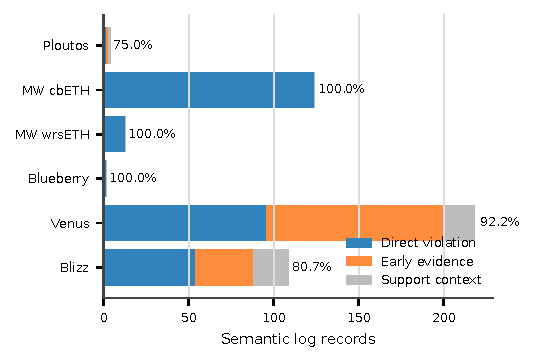
\includegraphics[width=\linewidth]{figures/eval_log_warning_breakdown.pdf}
    \caption{Positive log-warning composition by case. Direct violation and collateral-enabling early-evidence logs are warning targets; support-only context logs are replay context but not warning targets.}
    \label{fig:log-warning-breakdown}
\end{figure}

\paragraph{Results and analysis}
At case and transaction levels, \tool detects all six positive incidents and all 285 materialized impact transactions.
This result alone is not sufficient, because a curated positive set can make recall look perfect.
The log-level result is therefore more informative.
Direct violation recall is 100\% because every oracle anomaly, borrow impact, or liquidation impact in the positive trace triggers the intended replay constraint.
Incident-log warning recall includes direct violations and collateral-enabling supply logs, but it leaves support-only context logs in the denominator.
This yields 431 warnings over 470 positive semantic records, or 91.70\%: 291 direct violations and 140 collateral-enabling early-evidence records are flagged, while 39 support-only records are intentionally not treated as warning targets.

The six incidents exercise different parts of the same evidence-closure design.
For feed-binding failures, \tool must connect a protocol-side binding boundary to later lending impact, because the external feed itself may continue to report valid values.
For price-semantics failures, the signal is not a single abnormal topic; the replay record must bind wrapper or governance evidence to derivative-asset borrow or liquidation behavior.
For freshness failures, a stale oracle marker is only dangerous when it is followed by collateral-enabling supply and borrow impact under the same protocol state.
These differences explain why the metric is reported over semantic records rather than only over attack transactions.

The benign result is also reported with the unresolved evidence separated.
On 9,651 labelled benign samples, \tool produces no confirmed replayable attack false positives.
The result should still be interpreted with the excluded evidence in mind: 349 rows remain unknown after materialization and are not used in the false-positive denominator.

\paragraph{Answer to RQ1}
\tool detects all six historical incidents and all 285 materialized impact transactions.
At log level, it reports 431 warnings over 470 positive semantic records by combining 291 direct violations with 140 collateral-enabling early-evidence records.
On the benign set, the false-positive count is zero over 9,651 labelled benign samples, while 349 unresolved rows are excluded from the false-positive denominator.

\subsection{RQ2: Early Evidence Lead Time}

\paragraph{Experiment design}
To answer RQ2, we identify two timestamps for each positive case in the replay trace: the first dangerous oracle, configuration, or stale-price evidence, and the first downstream impact transaction.
The first evidence point may be a canonical pre-impact transaction, such as an oracle-binding update or stale oracle marker, or a validated semantic marker when the local artifact does not canonicalize the boundary transaction.
We keep these two statuses separate because they support different claims about deployable monitoring.

\paragraph{Metrics}
The primary metric is lead time, measured as the timestamp difference between the first dangerous evidence and the first downstream impact transaction.
Cases with canonical pre-impact transactions can support a transaction-level early-evidence claim.
Cases with semantic markers support retrospective detectability, but they are not used to claim that a concrete pre-impact transaction could have been automatically observed.

\begin{table}[t]
\centering
\caption{Early evidence lead time.}
\label{tab:lead}
\small
\begin{tabular}{llr}
\toprule
Case & Status & Lead time (s) \\
\midrule
Ploutos & Pre-attack tx observed & 12 \\
Moonwell cbETH & Pre-attack tx observed & 2 \\
Moonwell wrsETH & Semantic marker only & 1 \\
Blueberry & Semantic marker only & 63,971 \\
Venus LUNA & Pre-attack tx observed & 471 \\
Blizz LUNA & Pre-attack tx observed & 44,525 \\
\bottomrule
\end{tabular}
\end{table}

\paragraph{Results and analysis}
Table~\ref{tab:lead} reports the first dangerous evidence observed in each case.
Four cases have a canonical pre-impact transaction hash.
Two cases use validated semantic markers whose boundary transaction is not canonicalized in the local trace; we report them separately and do not claim a universal early warning.
The lead-time result should be interpreted as early evidence, not guaranteed prevention.
In Ploutos and Moonwell cbETH, the oracle boundary and first impact are close in time.
In Venus and Blizz, the stale marker appears minutes to hours before the first materialized borrow impact.
For Moonwell wrsETH and Blueberry, the local trace contains semantic markers rather than a canonical boundary transaction hash, so they are excluded from any claim that a concrete pre-impact transaction could have been automatically observed.

This distinction is important for operational interpretation.
A pre-impact boundary transaction means that a deployed monitor could have observed a concrete transaction before the first materialized impact.
A semantic marker means that the replay trace contains enough evidence to explain the failure, but the artifact does not establish a canonical transaction-level warning point.
Short lead times, such as Ploutos and Moonwell cbETH, are still useful for forensic reconstruction and runtime alerting, but they should not be presented as evidence that a protocol operator had enough time to intervene.

\paragraph{Answer to RQ2}
\tool observes pre-impact dangerous evidence for four of the six cases, with lead times ranging from 2 seconds to 44,525 seconds.
The remaining two cases are supported by validated semantic markers rather than canonicalized pre-impact transactions, so we report them as evidence of detectability but not as guaranteed early-warning opportunities.

\subsection{RQ3: Actor Localization}

\paragraph{Experiment design}
To answer RQ3, we collect the actor-bearing fields from replay records that participate in violated borrow or liquidation constraints.
Depending on the case, these fields include borrower, liquidator, transaction sender, recipient, or attacker-contract roles.
We compare the resulting candidate set against the known impact-role actors recorded in the case manifest.

\paragraph{Metrics}
We report the number of known impact actors, the number of localized candidates, and the number of matched actors for each case.
The metric evaluates role coverage in the materialized traces: a match means that the tool recovered the on-chain account appearing in an impact role.
It does not measure off-chain identity resolution or final fund-recipient tracing.

\begin{table}[t]
\centering
\caption{Actor localization.}
\label{tab:actors}
\small
\begin{tabular}{lrrr}
\toprule
Case & Known actors & Candidates & Matched \\
\midrule
Ploutos & 1 & 1 & 1 \\
Moonwell cbETH & 14 & 14 & 14 \\
Moonwell wrsETH & 2 & 2 & 2 \\
Blueberry & 2 & 2 & 2 \\
Venus LUNA & 12 & 12 & 12 \\
Blizz LUNA & 24 & 24 & 24 \\
\midrule
Total & 55 & 55 & 55 \\
\bottomrule
\end{tabular}
\end{table}

\paragraph{Results and analysis}
Across the six cases, the case manifest contains 55 known impact actors, and \tool reports all 55 as candidates.
This should not be read as legal attribution or full profit tracing.
The metric evaluates whether the replay constraints identify the on-chain accounts that appear in impact roles, such as borrower or liquidator.
It does not prove off-chain identity, nor does it guarantee that the first candidate is the ultimate beneficiary after swaps, bridges, or MEV payments.

The result depends on semantic role binding.
ABI decoding can reveal that an event contains an address, but it does not say whether that address is a borrower, liquidator, recipient, market, asset, feed, or implementation contract.
\tool treats actor localization as a replay output: once a violated constraint reaches a borrow or liquidation impact, the actor-bearing fields in that impact record become the candidate set.
This makes the metric suitable for incident triage and reproducible on-chain attribution, while leaving beneficiary tracing outside the scope of the experiment.

\paragraph{Answer to RQ3}
\tool matches all 55 known impact-role actors across the six cases.
This result shows that source-derived log roles are sufficient to recover borrower and liquidation actors in the materialized traces, but it should not be interpreted as off-chain identity resolution or complete profit-flow attribution.

\subsection{RQ4: Ablation Study}

\paragraph{Experiment design}
To answer RQ4, we rerun the same positive traces and benign samples under four ablated variants.
Each variant removes one part of the DSC-Guard evidence pipeline while preserving the same input artifacts.
The ABI-only parser decodes event fields without semantic role binding; the topic-only raw filter uses event topics without source-derived roles; the oracle-boundary-only variant observes oracle-side evidence without lending impact; and the impact-only variant observes lending impact without oracle-boundary evidence.

\paragraph{Metrics}
We compare the variants using replayable case recall, impact-transaction recall, actor recall, and benign warning rate.
These metrics are intentionally the same as in RQ1 and RQ3 so that improvements cannot be attributed to a different dataset or denominator.
The goal is not to reproduce full prior systems, but to isolate whether log semantics and evidence closure are necessary for this failure model.

\begin{table*}[t]
\centering
\caption{Ablation study.}
\label{tab:ablation}
\small
\begin{tabular}{lrrrr}
\toprule
Variant & Case recall & Impact tx recall & Actor recall & Benign warning rate \\
\midrule
Full \tool & 6/6 & 285/285 & 55/55 & 14/10,000 \\
ABI-only parser & 0/6 & 0/285 & 0/55 & 9,641/10,000 \\
Topic-only raw filter & 0/6 & 0/285 & 0/55 & 10,000/10,000 \\
Oracle boundary only & 0/6 & 0/285 & 0/55 & 10,000/10,000 \\
Impact only & 0/6 & 0/285 & 0/55 & 0/10,000 \\
\bottomrule
\end{tabular}
\end{table*}

Figure~\ref{fig:ablation-heatmap} visualizes the same ablation results as normalized rates.
It highlights that high replayable recall requires both semantic binding and evidence closure; topic-only and oracle-only variants see many benign warnings without producing replayable attack evidence.

\begin{figure}[t]
    \centering
    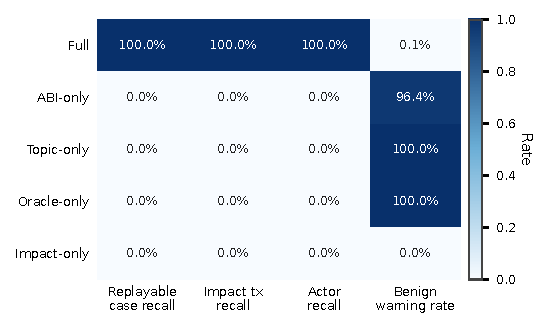
\includegraphics[width=\linewidth]{figures/eval_ablation_heatmap.pdf}
    \caption{Ablation heatmap. Removing semantic role binding or evidence closure eliminates replayable detection or produces high benign-warning volume.}
    \label{fig:ablation-heatmap}
\end{figure}

\paragraph{Results and analysis}
Table~\ref{tab:ablation} compares \tool with four read-only baselines.
The baselines intentionally remove semantic binding components while preserving the same positive and benign datasets.
The ablation highlights why the method needs log semantics rather than topics alone.
Topic-only and oracle-boundary-only baselines can observe oracle-like logs, but they cannot bind those logs to downstream lending impacts and therefore generate many warnings without replayable attack evidence.
The impact-only baseline observes borrow or liquidation events but cannot distinguish ordinary lending from oracle-consumption failure.
The ABI-only parser decodes event shapes but lacks asset/feed/actor/collateral semantics, so it cannot replay the constraints.
The full system is the only variant that connects oracle boundary, semantic anomaly, downstream lending impact, actor field, and temporal order.

The failure modes differ by baseline.
ABI-only parsing preserves typed fields but loses the role information required to decide whether a decoded address is an oracle feed, an affected asset, or an impact actor.
Topic-only and oracle-boundary-only variants observe many oracle-shaped logs, which explains their high benign-warning volume, but they cannot prove downstream lending impact.
The impact-only variant avoids those oracle-side warnings but collapses into ordinary lending monitoring, so it cannot distinguish a valid borrow from a borrow enabled by incorrect oracle consumption.

\paragraph{Answer to RQ4}
The ablation shows that no single observable layer is sufficient.
Replayable detection requires semantic role binding, oracle-boundary evidence, downstream lending impact, actor fields, and temporal order; removing any of these components either eliminates positive recall or produces many non-replayable benign warnings.

\section{Discussion}
\label{sec:discussion}

\subsection{Scope and Generality}

The evaluation covers six incidents and three failure classes.
This does not make \tool a universal oracle-attack detector, but it demonstrates that the same log-replay architecture applies beyond one feed collapse.
The common abstraction is not Chainlink-specific logs.
It is the evidence closure from oracle boundary or anomaly to protocol impact.

\subsection{Engineering Implications}

The results have three implications for developers of oracle-consuming lending protocols and analysis tools.
First, event design affects post-deployment analyzability: explicit oracle-binding, wrapper-update, market-entry, borrow, and liquidation events make evidence closure replayable, whereas silent configuration changes force tools to rely on incomplete traces.
Second, ABI-level decoding is not enough for semantic monitoring, because the same address-typed field may represent an asset, feed, borrower, liquidator, implementation, or market contract.
Third, oracle validation should be enforced at the consumer boundary; even when an external feed reports data successfully, the lending protocol can still consume it with incorrect identity, composition, or freshness semantics.

\subsection{Multi-Contract Interactions}

DeFi incidents often span proxies, oracles, lending markets, governance executors, and ERC20 tokens.
\tool represents multi-contract interactions through protocol-level semantic roles rather than a single-contract state machine.
For example, a stale oracle marker may come from a feed contract, a supply log from a market token, and a borrow log from a lending market.
The replay state connects them by asset identity, actor, temporal order, and protocol cluster.
This avoids global state explosion, but it depends on the availability and correctness of the selected evidence closure.
The approach is therefore suitable for bounded incident reconstruction and monitoring of known failure classes, not for whole-chain compositional verification.

\subsection{Generality and Porting Effort}

\tool is expected to generalize to unseen incidents within the three modeled failure classes, provided that the required evidence is observable in logs.
For example, a new stale-collateral incident in a Compound- or Aave-like lending market can reuse the freshness-handling constraint if the trace exposes an oracle stale marker, collateral supply, borrow impact, actor field, and temporal order.
Similarly, a new feed-binding failure can reuse the identity-mismatch constraint once the protocol's asset, feed, and lending-impact logs are bound to semantic roles.
In this setting, generalization is not based on memorizing the six cases; it comes from replaying the same failure-class invariant over a new protocol trace.

Porting to a new protocol still requires engineering work.
The main task is semantic role binding: identifying which events or decoded receipt flows represent oracle boundaries, supply or mint actions, borrow actions, liquidation actions, assets, feeds, markets, actors, and amounts.
For protocols in a familiar lending family, this is mostly mapping existing event schemas to the roles already used by the replay engine.
For derivative-asset or oracle-wrapper designs, the analyst must also confirm the intended price-composition invariant, because the correct formula may be protocol-specific.
When source code, ABI metadata, or protocol-level events are missing, the tool can still preserve receipt-flow evidence, but the case may be downgraded to incomplete or unknown rather than treated as a fully replayable detection.

\tool does not automatically detect arbitrary new oracle-consumption failure classes.
If a future incident violates a business invariant not covered by feed identity, price composition, freshness, or bad-collateral borrowing, a new replay constraint must be specified.
The reusable part is the pipeline: source mining, ABI/log binding, ordered replay trace generation, K-style constraint checking, and actor extraction.
We therefore report the required engineering tasks rather than claiming a fixed number of person-hours; a controlled time-and-motion study of porting effort is left for future work.

\subsection{Logs-Only Blind Spot}

The strongest limitation is that not every state change emits a log.
If a protocol changes an oracle path silently through an internal call or stores a value without emitting an event, a log-driven state machine can miss the transition.
Source-code mining can reveal that such silent transitions exist, but the runtime trace may still be incomplete.
Therefore, \tool should be used as a log-semantics replay tool, not as a sound complete verifier for all EVM state.

\subsection{Threats to Validity}

The positive set is curated from known incidents, so the case-level recall should not be interpreted as population-level recall over all DeFi failures.
The benign set is stronger than random negatives because it is case-aware, but 349 rows remain unknown after materialization.
We exclude those rows from the false-positive denominator and report the labelled benign denominator separately.
The benign set also should not be interpreted as a representative sample of all deployed DeFi protocols.
It covers the four chains and oracle/lending surfaces connected to the evaluated cases, and its purpose is to test whether \tool avoids warnings on logs that resemble the positive incidents without closing the oracle-consumption failure loop.
Some loss estimates are partial.
For example, Ploutos uses receipt-flow impact rather than fully ABI-decoded protocol loss, and Blizz's known borrowed USD covers 76.15\% of the public loss reference.

\section{Related Work}
\label{sec:related}

\paragraph{Smart-contract analysis and formal verification}
Smart-contract research has long treated contract security as a program-analysis, verification, and tooling problem.
Static and hybrid analyzers recover contract-level properties from source code, bytecode, or intermediate representations, including Slither's Solidity analysis \cite{feist2019slither}, precise EVM control-flow reconstruction \cite{pasqua2023cfg}, heterogeneous vulnerability learning \cite{cai2024finegrained}, and empirical studies of Solidity bug fixes \cite{wang2023soliditybugfixes}.
Formal approaches provide EVM or Solidity semantics, model checking, and temporal property checking, including KEVM \cite{hildenbrandt2018kevm}, Solidity executable semantics \cite{jiao2020semantic}, ZEUS \cite{kalra2018zeus}, VeriSol \cite{wang2019formal}, FairCon \cite{liu2020towards}, and SmartPulse \cite{stephens2021smartpulse}; recent surveys and JSS studies summarize this broader vulnerability-detection landscape \cite{vidal2024slr,iuliano2026slr,soud2025soley,chang2026codespeak}.
These works are closest to \tool in their use of source semantics and formal reasoning, but they primarily target generic contract vulnerabilities, complete language semantics, or contract-local temporal properties.
\tool instead uses static analysis to derive log roles and then checks historical oracle-consumption evidence across protocol contracts.

\paragraph{Oracle, DeFi price security, and protocol-composition analysis}
Oracle and DeFi security studies have examined both oracle infrastructure and price-manipulation behavior.
Early work characterizes blockchain oracle designs and risks, including authenticated data feeds, trustworthy oracle architectures, Chainlink usage, and DeFi oracle deployment practices \cite{zhang2016town,al2020trustworthy,kaleem2021demystifying,liu2021first}; DArcher studies on-chain/off-chain synchronization bugs in decentralized applications \cite{zhang2021dharcher}.
For detection, VeriOracle identifies unexpected price-feed usage from smart-contract source code \cite{mo2023toward}, while DeFiRanger, DeFiScope, and DeFiTainter target price manipulation, inferred price models, or manipulation vulnerabilities in DeFi protocols \cite{wu2021defiranger,zhong2025defiscope,kong2023defitainter}.
Other studies analyze flash-loan attacks, MEV, front-running, high-frequency trading, automated economic-security analysis, and profit-generating transaction discovery \cite{qin2021attacking,daian2020flash,torres2021frontrunner,zhou2021high,babel2021clockwork,zhou2021just}.
These works mostly reason about source-level feed misuse, market-side price movement, transaction-level token flows, or global compositional economics.
\tool is complementary: the external price may be valid, but the lending consumer violates identity, composition, or freshness semantics, and the evidence must connect oracle-boundary logs to downstream lending impact.

\paragraph{Log analysis and blockchain forensic evidence}
Classical log-analysis research studies parsing, template inference, anomaly detection, and reliability engineering over system logs \cite{he2021survey,he2017drain,le2022log}.
Representative techniques include semantic log parsing \cite{huo2021semparser}, n-gram parsing \cite{dai2020logram}, robust log anomaly detection \cite{zhang2019robust}, and deep-learning-based sequence anomaly detection \cite{du2017deeplog}.
These methods usually operate on textual or semi-structured system logs, whereas EVM logs are typed receipt records with indexed topics, ABI-encoded fields, transaction order, and emitting contracts.
However, ABI-only blockchain log parsing still recovers field values rather than semantic roles: an address may be an actor, asset, feed, market, proxy, implementation, or recipient.
\tool therefore treats logs as forensic evidence only after source-derived role binding and evidence closure, producing replayable semantic records rather than raw topic matches or transaction-level token-balance summaries.

\section{Conclusion}

This paper presents \tool, a semantic log replay tool for detecting price-oracle consumption failures in EVM lending protocols.
By narrowing the scope from general DON attacks to feed-binding, price-composition, and freshness-handling failures, the method becomes empirically testable and technically precise.
On six historical incidents and 10,000 case-aware benign samples, \tool detects all known incidents and impact transactions, achieves 91.70\% incident-log warning recall, and produces no false positives among 9,651 labelled benign samples.
The ablation study shows that raw topics, ABI-only parsing, and single-side oracle or impact visibility are insufficient without semantic binding and replay constraints.
The method is not a complete EVM verifier and cannot see unlogged state changes, but it provides a practical software-engineering technique for reconstructing and checking oracle-consumption behavior from historical smart-contract logs.

\section*{Data Availability}
The artifact snapshot is available at \url{https://github.com/YifanMo/DSC-guard}.
It contains the reproducibility scripts, case configuration, semantic IR, generated K-style replay semantics, materialized replay traces, benign sample manifests, evaluation summaries, result reports, and paper tables used in this manuscript.
Large raw RPC/explorer caches, raw receipt aggregates, source caches, and debug traces are excluded from the Git snapshot because they are large and can be regenerated by the scripts with user-provided API keys.

\section*{Acknowledgments}
Omitted for anonymity.

\bibliographystyle{elsarticle-num}
\bibliography{references}

\end{document}
